\documentclass[conference]{IEEEtran}

\usepackage{algorithm}
\usepackage{algorithmic}
\usepackage{pgfplots}
\usepackage{cite}
\usepackage{amsmath}
\interdisplaylinepenalty=2500
\usepackage{array}
\usepackage{tikz}
\usetikzlibrary{positioning}
\usetikzlibrary{calc}
\usetikzlibrary{backgrounds}

\tikzset{
    between/.style args={#1 and #2}{
    	at = ($(#1)!0.5!(#2)$)
    }
}

\hyphenation{}

\begin{document}

\makeatletter
\newcommand\fs@spaceruled{\def\@fs@cfont{\bfseries}\let\@fs@capt\floatc@ruled
  \def\@fs@pre{\vspace{.5em}\hrule height.8pt depth0pt \kern2pt}%
  \def\@fs@post{\kern2pt\hrule\relax}%
  \def\@fs@mid{\kern2pt\hrule\kern2pt}%
  \let\@fs@iftopcapt\iftrue}
\makeatother

\title{Performance Analysis of SDN and NFV enabled Mobile Cloud Computing}

\author{\IEEEauthorblockN{Joseph Billingsley\IEEEauthorrefmark{1},
Wang Miao\IEEEauthorrefmark{1},
Ke Li\IEEEauthorrefmark{1},
Geyong Min\IEEEauthorrefmark{1}, 
 and Nektarios Georgalas\IEEEauthorrefmark{2}}
\IEEEauthorblockA{\IEEEauthorrefmark{1}Department of Computer Science,
University of Exeter, UK\\
Email: \{jb931, wang.miao, k.li, g.min\}@exeter.ac.uk}
\IEEEauthorblockA{\IEEEauthorrefmark{2}Research and Innovation, British Telecom, UK\\
Email: nektarios.georgalas@bt.com}}
 
\maketitle

\begin{abstract}
Mobile Cloud Computing (MCC) is regarded as a promising method to increase the data storage and enhance the processing power of mobile devices. Technologies such as Software Defined Networking (SDN) and Network Function Virtualisation (NFV) will be deployed in MCC to simplify the network management and accelerate mobile service deployment. There have been some interesting research findings in the literature regarding the performance of SDN and NFV in MCC, however most of the existing work only considers these technologies in isolation and pays little attention to their cooperative and complementary relations in practical deployments. In order to achieve a deeper understanding of future MCC, a comprehensive analytical model is developed in this work to investigate the performance of MCC in the presence of both NFV service chains and SDN networks. The proposed model is capable of capturing the interactions between SDN and NFV when they share the same underlying physical infrastructure. The end-to-end latency is derived for different scales of service deployments and network configurations. Comprehensive simulation experiments are conducted and the results demonstrate that the proposed analytical model corresponds well with the simulation experiments. In addition, we show how the analytical model can be a useful tool to investigate the impact of centralised SDN control on the performance of NFV traffic transmission. 
\end{abstract}

% !TeX root=main.tex

\section{Introduction}
\label{sec:introduction}

Next generation communications networks are faced with scaling to support greater expectations and usage of existing services \cite{AndrewsBCHLSZ14} whilst simultanously supporting demanding new use cases such as the internet of things, smart cities and virtual and augmented reality \cite{GSA15}. Two technologies that have emerged as part of the solution to these problems are Network Function Virtualisation (NFV) and Software Defined Networking (SDN).

Fast analytical models allow for evaluation and optimisation of large scale networks. Existing research into analytical models of NFV and SDN has focussed on them in isolation. Longo et al. \cite{LongoDBS15} constructed a model of the reliability of a two layer hierarchical SDN controller. Similarily, Azodolmolky et al. \cite{AzodolmolkyWY13} also examine the two layer SDN controller but use network calculus to determine the worst case delay incurred by visiting it and the minimum buffer size required to prevent packet loss given the highest load. Wang et al. \cite{MiaoMWWH16} produce a more accurate SDN model by considering the bursty and correlated arrivals of packets and a high and low priority queue at an SDN enabled switch.

Similarily in NFV modeling, Prados-Garzon et al. \cite{Prados-GarzonAR17} produced a detailed model of a single VNF which is composed of several VNF components and calculate the average response time of the VNF. Gebert et al. \cite{GebertZLST16} analysed a single VNF in even more detail by modelling the packet processing process of a Linux x86 system. Their model estimates latency and packet loss within the 95\% confidence interval of lab testing of a real world server. To the best of our knowledge, only Fahmin et al. \cite{FahminLHLS17} considered both NFV and SDN. They analysed the performance of two methods of combining SDN and NFV in the network. However they consider a simplfied network with only a single switch and VNF.

In this work we strike a middle ground between existing approaches by considering all relevant aspects of the network at an appropriate level of detail. To the best of our knowledge we are the first researchers to produce an integrated model that can consider the impact of the SDN controller, NFV in a practical network topology. The key contributions of this paper are:

\begin{itemize}
\item An efficient analytical model for a next generation NFV enabled network containing a centralised SDN controller using M/M/1 queues.
\item Extensions for different length service chains and multiple services in the same network.
\item An extension to model VNFs that reduce packet rate as part of a service chain.
\end{itemize}

The rest of this paper is organised as follows. \pref{sec:preliminaries} reviews the preliminaries that are useful for understanding the subsequent sections. In \pref{sec:analytical_model} we derive the analytical model. \pref{sec:validation} validates this model with extensive simulation experiments. Finally \pref{sec:conclusions} concludes the paper, explores the implications of the models and examines future research directions.

% !TeX root=main.tex

\section{Network Architecture}
\label{sec:preliminaries}

\begin{figure}

\centering

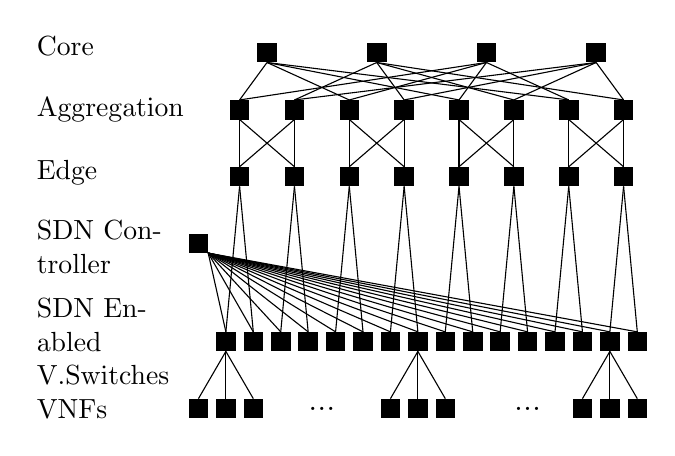
\begin{tikzpicture}[
every node/.style={node distance=6mm and 1mm},
server/.style={rectangle, draw=black, fill=black, node distance=10mm and 1mm},
edge/.style={rectangle, draw=black, fill=black},
agg/.style={rectangle, draw=black, fill=black},
core/.style={rectangle, draw=black, fill=black},
sdn/.style={rectangle, draw=black, fill=black,node distance=10mm and 1mm},
vm/.style={rectangle, draw=black, fill=black},
]

% Servers
\node[server]      (S1)                       {};
\node[server]      (S2)        [right=of S1]  {};
\node[server]      (S3)        [right=of S2]  {};
\node[server]      (S4)        [right=of S3]  {};
\node[server]      (S5)        [right=of S4]  {};
\node[server]      (S6)        [right=of S5]  {};
\node[server]      (S7)        [right=of S6]  {};
\node[server]      (S8)        [right=of S7]  {};
\node[server]      (S9)        [right=of S8]  {};
\node[server]      (S10)       [right=of S9]  {};
\node[server]      (S11)       [right=of S10] {};
\node[server]      (S12)       [right=of S11] {};
\node[server]      (S13)       [right=of S12] {};
\node[server]      (S14)       [right=of S13] {};
\node[server]      (S15)       [right=of S14] {};
\node[server]      (S16)       [right=of S15] {};

\node[text width=2cm] at (-1.4, 0)  {SDN Enabled V.Switches};

% VMs
\node[vm]      (V1)        [below=of S1]  {};
\node[vm]      (V2)        [below=of S1, left=of V1]  {};
\node[vm]      (V3)        [below=of S1, right=of V1]  {};

\node[vm]      (V4)        [below=of S8]  {};
\node[vm]      (V5)        [below=of S8, left=of V4]  {};
\node[vm]      (V6)        [below=of S8, right=of V4]  {};

\node[vm]      (V7)        [below=of S15]  {};
\node[vm]      (V8)        [below=of S15, left=of V7]  {};
\node[vm]      (V9)        [below=of S15, right=of V7]  {};

\node[text width=0.8cm] at (-2, -.86)  {VNFs};
\node [between=V1 and V4] {\large ...};
\node [between=V6 and V7] {\large ...};

% SDN Controller
\node[text width=2cm] at (-1.4, 1.2)  {SDN Controller};
\node[sdn]      (SC1)      	 [above left=of S1] {};

% Edge/ToR
% This weird hack stops Tikz from placing the points at the same level as the SDN Controller
%\node[bug_example]      (test)      [above=of SC1, between=S15 and S16] {};

\node[text width=0.8cm] at (-2, 2.15)  {Edge};
\node[] 		 (H1) 		 [above=of SC1] {};
\node[] 		 (H2) 		 [between=S1 and S2] {};
\node[] 		 (H3) 		 [between=S3 and S4] {};
\node[] 		 (H4) 		 [between=S5 and S6] {};
\node[] 		 (H5) 		 [between=S7 and S8] {};
\node[] 		 (H6) 		 [between=S9 and S10] {};
\node[] 		 (H7) 		 [between=S11 and S12] {};
\node[] 		 (H8) 		 [between=S13 and S14] {};
\node[] 		 (H9) 		 [between=S15 and S16] {};

\node[edge]      (E1)        [at = (H1 -| H2)] {};
\node[edge]      (E2)        [at = (H1 -| H3)] {};
\node[edge]      (E3)        [at = (H1 -| H4)] {};
\node[edge]      (E4)        [at = (H1 -| H5)] {};
\node[edge]      (E5)        [at = (H1 -| H6)] {};
\node[edge]      (E6)        [at = (H1 -| H7)] {};
\node[edge]      (E7)        [at = (H1 -| H8)] {};
\node[edge]      (E8)        [at = (H1 -| H9)] {};

% Aggregate
\node[text width=0.8cm] at (-2, 2.95)  {Aggregation};
\node[agg]      (A1)        [above=of E1] {};
\node[agg]      (A2)        [above=of E2] {};
\node[agg]      (A3)        [above=of E3] {};
\node[agg]      (A4)        [above=of E4] {};
\node[agg]      (A5)        [above=of E5] {};
\node[agg]      (A6)        [above=of E6] {};
\node[agg]      (A7)        [above=of E7] {};
\node[agg]      (A8)        [above=of E8] {};

% Core
\node[text width=0.8cm] at (-2, 3.75)  {Core};
\node[core]      (C1)        [above=of A1,  between=A1 and A2]  {};
\node[core]      (C2)        [above=of A3,  between=A3 and A4]  {};
\node[core]      (C3)        [above=of A5,  between=A5 and A6]  {};
\node[core]      (C4)        [above=of A7,  between=A7 and A8]  {};

%Lines
\draw[-] (V1.north)  -- (S1.south);
\draw[-] (V2.north)  -- (S1.south);
\draw[-] (V3.north)  -- (S1.south);

\draw[-] (V4.north)  -- (S8.south);
\draw[-] (V5.north)  -- (S8.south);
\draw[-] (V6.north)  -- (S8.south);

\draw[-] (V7.north)  -- (S15.south);
\draw[-] (V8.north)  -- (S15.south);
\draw[-] (V9.north)  -- (S15.south);

\draw[-] (S1.north)  -- (E1.south);
\draw[-] (S2.north)  -- (E1.south);
\draw[-] (S3.north)  -- (E2.south);
\draw[-] (S4.north)  -- (E2.south);
\draw[-] (S5.north)  -- (E3.south);
\draw[-] (S6.north)  -- (E3.south);
\draw[-] (S7.north)  -- (E4.south);
\draw[-] (S8.north)  -- (E4.south);
\draw[-] (S9.north)  -- (E5.south);
\draw[-] (S10.north) -- (E5.south);
\draw[-] (S11.north) -- (E6.south);
\draw[-] (S12.north) -- (E6.south);
\draw[-] (S13.north) -- (E7.south);
\draw[-] (S14.north) -- (E7.south);
\draw[-] (S15.north) -- (E8.south);
\draw[-] (S16.north) -- (E8.south);

\draw[-] (S1.north)  -- (SC1.south east);
\draw[-] (S2.north)  -- (SC1.south east);
\draw[-] (S3.north)  -- (SC1.south east);
\draw[-] (S4.north)  -- (SC1.south east);
\draw[-] (S5.north)  -- (SC1.south east);
\draw[-] (S6.north)  -- (SC1.south east);
\draw[-] (S7.north)  -- (SC1.south east);
\draw[-] (S8.north)  -- (SC1.south east);
\draw[-] (S9.north)  -- (SC1.south east);
\draw[-] (S10.north) -- (SC1.south east);
\draw[-] (S11.north) -- (SC1.south east);
\draw[-] (S12.north) -- (SC1.south east);
\draw[-] (S13.north) -- (SC1.south east);
\draw[-] (S14.north) -- (SC1.south east);
\draw[-] (S15.north) -- (SC1.south east);
\draw[-] (S16.north) -- (SC1.south east);

\draw[-] (E1.north)  -- (A1.south);
\draw[-] (E2.north)  -- (A2.south);
\draw[-] (E3.north)  -- (A3.south);
\draw[-] (E4.north)  -- (A4.south);
\draw[-] (E5.north)  -- (A5.south);
\draw[-] (E6.north)  -- (A6.south);
\draw[-] (E7.north)  -- (A7.south);
\draw[-] (E8.north)  -- (A8.south);

\draw[-] (E1.north)  -- (A2.south);
\draw[-] (E2.north)  -- (A1.south);
\draw[-] (E3.north)  -- (A4.south);
\draw[-] (E4.north)  -- (A3.south);
\draw[-] (E5.north)  -- (A6.south);
\draw[-] (E6.north)  -- (A5.south);
\draw[-] (E7.north)  -- (A8.south);
\draw[-] (E8.north)  -- (A7.south);

\draw[-] (A1.north)  -- (C1.south);
\draw[-] (A1.north)  -- (C3.south);
\draw[-] (A2.north)  -- (C2.south);
\draw[-] (A2.north)  -- (C4.south);
\draw[-] (A3.north)  -- (C1.south);
\draw[-] (A3.north)  -- (C3.south);
\draw[-] (A4.north)  -- (C2.south);
\draw[-] (A4.north)  -- (C4.south);
\draw[-] (A5.north)  -- (C1.south);
\draw[-] (A5.north)  -- (C3.south);
\draw[-] (A6.north)  -- (C2.south);
\draw[-] (A6.north)  -- (C4.south);
\draw[-] (A7.north)  -- (C1.south);
\draw[-] (A7.north)  -- (C3.south);
\draw[-] (A8.north)  -- (C2.south);
\draw[-] (A8.north)  -- (C4.south);

\end{tikzpicture}

\caption{An example SDN and NFV enabled fat-tree network with 4 ports for each hardware switch and 3 for the virtual switches.}

\label{fig:network_topology}

\end{figure}

As shown in Fig. \ref{fig:network_topology}, we abstract a network architecture where multiple NFV chains are deployed and linked by a virtualised SDN architecture. With NFV deployment, a service is provided in the form of a service chain which is formed by several VNFs. The packets pass through each of the VNFs in sequence. Based on the performance requirements, service chains are composed of different numbers and types of VNFs. In the abstracted network architecture, multiple NFV chains can simultaneously coexist in the datacenter.

Service chains may be physically distributed over the datacenter. Communication between servers in the datacenter is provided by the interconnection network. The fat-tree or folded-Clos topology is currently the most common topology used for interconnection networks in datacentres \cite{Cisco18}. The fat-tree topology (see Fig. \ref{fig:network_topology}) is formed of three layers of switches: Core, Aggregation and Edge. Switches at the edge layer are additionally connected to servers. In an NFV enabled datacentre each of these servers contains a virtual switch which manages one or more VNFs.

The fat-tree topology is dependent upon the number of ports at each switch. We define $k$ as the number of ports for each physical switch and $k_{vsw}$ as the number of ports for each virtual switch. There are $(k/2)^2$ core switches. Each core switch connects to one switch in each of $k$ pods. Each pod contains two layers (aggregation and edge) of $k/2$ switches. Each edge switch is connected to each of the $k/2$ aggregation switches of the pod. Each edge switch is connected to $k/2$ servers. Each server contains a virtual switch connected to $k_{vsw}$ VNFs. This topology results in $n=(k^3/4) \cdot k_{vsw}$ VNFs.

In an SDN enabled datacentre an SDN controller provides centralised management, instructing the switches how to direct traffic to ensure it takes an efficient route to its destination. Each SDN enabled switch has a flow table maintained by the controller containing instructions on where to send received packets. This table may not be large enough to contain instructions for all possible destinations. If the local switch receives a packet that it does not have matching instructions for, it must request instructions from the controller. As a result a portion of the packets in the datacentre visit the controller. For this work we consider an SDN architecture where only the virtual switches connect to the SDN controller. This architecture is representative of those used in industry, most notably a comparable architecture is used in VMWare's NSX solution \cite{VMW18}.


% !TeX root=main.tex

\section{Analytical Model}
\label{sec:analytical_model}

\subsection{Assumptions}
The analytical model is based on the following assumptions which are commonly accepted in the literature \cite{}. Assumption 3 is based on the high speed of data centre interconnection networks and the short distances between components.

\begin{enumerate}
\item At each VNF, messages are generated according to an independant Poisson process with a mean rate of $\lambda$ messages a cycle. Furthermore, message destinations are uniformly distributed across the VNFs.
\item At each network component messages are serviced according to an independant Poisson process with a mean rate of $\mu$ messages a cycle.
\item The time taken for a message to travel between network components in negligible.
\item The SDN controller ensures messages take the shortest path between the two destinations and that messages are evenly distributed over the switches in the network.
\item Queues at each network component have infinite capacity.
\item Messages sent from a VNF to VNFs on other servers, may need to visit the SDN controller with probability $p_{sdn\_user}$. The same does not apply to messages arriving at a server as the route to the destination will be known.
\end{enumerate}

The mean message latency of the network can be calculated as the sum of the waiting time at each network component a message visits. As a result of the network architecture, messages will take shorter paths to visit VNFs under the same server, edge switch or pod. Consequently, the traffic arriving at servers at each layer in the network will also vary. The mean message latency for a single hop service chain can hence be calculated as:

\begin{equation} 
\label{eq:mean_latency}
\begin{split}
L&atency_{base} = ((w_{vm} + w_{sdn} + w_{srv}) \cdot p_{srv} \\
		&+ (w_{vm} + w_{sdn} + 2w_{srv} + w_{edge}) \cdot p_{edge} \\
	 	&+ (w_{vm} + w_{sdn} + 2w_{srv} + 2w_{edge} + w_{agg}) \cdot p_{agg} \\
	 	&+ (w_{vm} + w_{sdn} + 2w_{srv} + 2w_{edge}  \\
		& \;\;\;\quad\qquad\quad\qquad + 2w_{agg} + 2w_{core})\cdot p_{core})
\end{split}
\end{equation}

Where $w_{vm}$, $w_{sdn}$, $w_{srv}$,$w_{edge}$,$w_{agg}$, $w_{core}$ represent the average time spent in a VM, the SDN controller, a virtual, edge, aggregate and core switch respectively. Similarily $p_{srv}$, $p_{edge}$, $p_{agg}$ and $p_{core}$ represent the probability that the highest level a message which reach is a virtual, edge, aggregate or core switch respectively. The remainder of this section will deduce these values for arbitary settings of $k$ and $k_vm$.

\subsection{Probability of Highest Level}
As messages will always take the shortest path, a message will visit only a virtual switch if the destination VM is in under the same virtual switch as the source. Given $n=k^3/4 \cdot k_{vm}$ total VMs:

\begin{equation}
p_{vm} = \frac{k_{vm} - 1}{n - 1}
\end{equation}

Similarily the probability of a message visiting at highest an edge switch is the proportion of destinations that are under the edge switch, excluding those destinations that could be visited via a shorter route.

\begin{equation}
p_{edge} = \frac{(k/2) \cdot k_{vm} - k_{vm}}{n - 1}
\end{equation}

This same techinque can be used to find the remaining probabilities:

\begin{align}
&p_{agg} = \frac{(k/2)^2 \cdot k_{vm} - (k/2) \cdot k_vm}{n - 1} \\ \nonumber \\
&p_{core} = \frac{n - (k/2)^2 \cdot k_{vm}}{n - 1}
\end{align}

Finally we can calculate the probability $p_{sdn}$ by excluding all messages that will not leave the server:

\begin{equation}
p_{sdn} = p_{sdn\_user} \cdot (1 - p_{vm})
\end{equation}

\subsection{Calculation of Mean Waiting Time}
To determine the mean waiting time at each network component, we model each component as a M/M/1 queue where the mean waiting time is calculated as \cite{}:

\begin{equation}
\label{eq:MM1_time_in_network}
MM1(\mu, \lambda_{nc}) = \frac{1}{\mu - \lambda_{nc}}
\end{equation}

Where $nc$ is the network component under question. Despite messages being distributed evenly across switches in each layer by the SDN controller, the arrival rate, $\lambda_{nc}$, will be different for each layer as not all messages will visit all layers.

As destinations are evenly distributed over the VNFs, all VNFs will send an equal proportion of messages to all others:

\begin{equation}
\label{eq:arr_vnf}
\begin{split}
\lambda_{vm} &= \frac{n - 1}{n - 1} \cdot \lambda \\
			 &= \lambda
\end{split}
\end{equation}

A portion of the messages being produced by every VNF will require the SDN controller to be consulted:

\begin{equation}
\label{eq:arr_sdn}
\lambda_{sdn} = n \cdot p_{sdn} \cdot \lambda
\end{equation}

Servers can receive messages from three sources: generated from VNFs it is running, received from other VNFs and reflected messages that it had sent to the SDN. Following the same format:

\begin{equation}
\label{eq:arr_srv}
\begin{split}
\lambda_{srv} &= k_{vm} \cdot \lambda \\
			  &+ (n - k_{vm}) \cdot  \frac{k_{vm}}{n - 1} \cdot \lambda \\
			  &+ k_{vm} \cdot \lambda \cdot p_{sdn}
\end{split}
\end{equation}

Where line two can be understood as the number of VNFs that are not hosted by the server, sending an equal proportion of their messages to each of the VNFs hosted by the server.

Note that the SDN controller does not affect switches as the portion of messages that are sent to the controller are not sent to higher switches till later cycles and that this absence is filled by messages returned from the SDN controller from earlier cycles. 

The arrival rate for the edge switches can then be deduced in the same way. Following the same order:

\begin{equation}
\label{eq:arr_edge}
\begin{split}
\lambda_{edge} &= ((k/2) \cdot k_{vm}) \cdot (n - k_{vm}) \cdot \frac{1}{n - 1} \cdot \lambda \\
			   &+ (n - ((k/2) \cdot k_{vm}) \cdot \frac{(k/2) \cdot k_{vm}}{n - 1} \cdot \lambda 
\end{split}
\end{equation}

The same principle can also be followed for the aggregate switches only now all traffic will be split between each aggregate switch in the pod. In the same order:

\begin{equation}
\label{eq:arr_agg}
\begin{split}
\lambda_{agg} &= (k/2)^2 \cdot k_{vm} \cdot \frac{n - (k_{vm} \cdot (k/2))}{n - 1} \cdot \frac{\lambda}{k/2} \\
			  &+ n - ((k/2)^2 k_{vm}) \cdot \frac{(k/2)^2 \cdot k_{vm}}{n - 1} \cdot \frac{\lambda}{k/2}
\end{split}
\end{equation}

Finally, as all VNFs are descendants of all core switches the arrival rate at each core can be calculated as the portion of messages arriving at a core switch, split evenly between each of the core switches.

\begin{equation}
\label{eq:arr_core}
\lambda_{core} = p_{core} \cdot n \cdot  \frac{1}{(k / 2)^2} \cdot  \lambda
\end{equation}

By substituting \ref{eq:arr_vnf} to \ref{eq:arr_core} for the arrival rates at each network component into \ref{eq:MM1_time_in_network} for the average waiting time we can calculate the latency incurred when visiting a network component, $w_{nc}$, for all network components except for the SDN controller.

When a message is sent to the controller it will incurr added latency both waiting at the controller and waiting at the server again when it returns. The expectation of the waiting time incurred by the SDN controller is:

\begin{equation}
w_{sdn} = (MM1(\mu, \lambda_{sdn}) + w_{srv}) * p_{sdn}
\end{equation}

\subsection{Mean Latency of Long Services and Many Services}
As discussed in the preliminary section telecommunications services are typically composed from several network functions that pass messages from one to the other. As a result messages persist in the network for a longer period of time. 

Consider a situation where each VNF send a message to an adjacent network function every cycle, under the same server or otherwise, so that all network functions will receive a message each cycle. Consider also that we have a service chain of three network function so that messages will be required to make two hops. 

After the first cycle all messages will have sent and received one message. After the second cycle all messages will have sent two messages, forwarding the one received in the previous step and a new message from this cycle, and also received two messages, a message with no hops remaining and one with one hop remaining. At the third cycle one message will be destroyed having completed, leaving one message to be forwarded and one new message created for each VNF. The net result is that on average each VNF is producing 2 messages per cycle.

We can extend this intuition to arbitary length chains. Applying this back to the original analytical model we get:

\begin{equation}
\lambda = \lambda_{new} \cdot (len(chain_i) - 1)
\end{equation}

where $\lambda_{new}$ is the average number of new messages that are generated each cycle, $len$ is the number of network functions that compose a given service chain and $chain_i$ is the service being modelled.

We can further extend this to several services, each of which may have different numbers of network functions. If a given message has probability $p(chain_i)$ of belonging to a particular service the average number of hops that a message persists for and hence the impact on the production rate can be calculated as:

\begin{equation}
\lambda = \lambda_{new} \sum_{i=1}^{ns} p(chain_i) \cdot (len(chain_i) - 1)
\end{equation}

where $ns$ is the number of different services and $\sum_{i=1}^{ns} p(chain_i) = 1$.

Finally we must also consider that messages that require several hops must also traverse the network several times. We can extend \pref{eq:mean_latency} by multiplying it by the average number of hops in the network considering each service:

\begin{equation}
Latency = Latency_{base} \cdot \sum_{i=1}^{ns} p(chain_i) \cdot (len(chain_i) - 1)
\end{equation}

\subsection{Mean Latency with Filtering VNFs}
We make one final extension for the case where one or more network functions in a service may not forward all of the messages that they receive. As a result subsequent network functions in a service chain have lower production rates. 

We can use the same conceptual model as before to solve this. Consider a situation where we have a service chain with 4 VNFs with 2 filtering VNFs that remove 50\% of the traffic, as illustrated in \ref{}. After the first cycle all VNFs will have sent and received 1 message. After the second cycle all VNFs will have sent at least one message, and half of the VNFs will have forwarded another message bringing the average production rate to 1.5. After the first cycle all VNFs will have produced at least 1 message, another half will have forwarded the message received in the previous cycle and a quarter will have forwarded the message sent in the first cycle bringing the average production rate to 1.75.

We can extend this process to several services in the same manner as before by averaging the production rates of each service. The complete algorithm for calculating the production rate considering all aspects is as follows:

\begin{algorithmic}[1]
\FOR{$i = 1:ns$} 
\STATE{

$multiplier \leftarrow 1$

\FOR{$j = 1:len(chain_i$)}
\STATE{

$multiplier \leftarrow multiplier \cdot chain_i(j)$ \\
$\lambda_i  \leftarrow \lambda_i + \lambda_{new} * multiplier$

}
\ENDFOR
}

\ENDFOR

\STATE $\lambda \leftarrow \sum_{i=1}^{ns} \lambda_i \cdot p(chain_i)$

\end{algorithmic}

% !TeX root=main.tex

% Different Number of Ports
\begin{figure*}
	\centering
	\begin{minipage}[b]{.49\textwidth}
		% 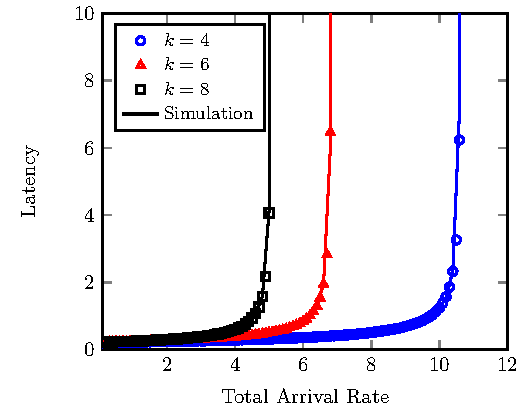
\includegraphics[width=\linewidth]{graphs/num_ports}
		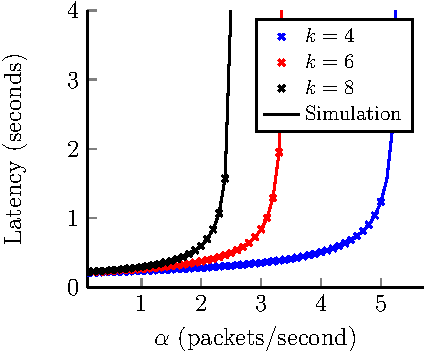
\includegraphics[width=\linewidth]{graphs/num_ports-crop}
		\caption{Latency predicted by the model and simulation for different numbers
		of ports ($N_s=1$, $K_i=2$, $k={8,16,24}$, $k_v=2$, $p_m=0$).}
		\label{fig:num_ports}
	\end{minipage}
	\hfill
	\begin{minipage}[b]{.49\textwidth}
		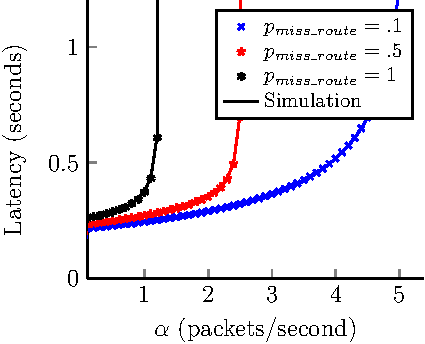
\includegraphics[width=\linewidth]{graphs/diff_sdn-crop}
		\caption{Latency predicted by the model and simulation for different miss rates ($N_s=1$, $K_i=2$, $k=4$, $k_v=2$, $p_m={0.1,0.5,1.0}$).}
		\label{fig:sdn_perc}
	\end{minipage}

	\vspace{2mm}

	\begin{minipage}[b]{.49\textwidth}
		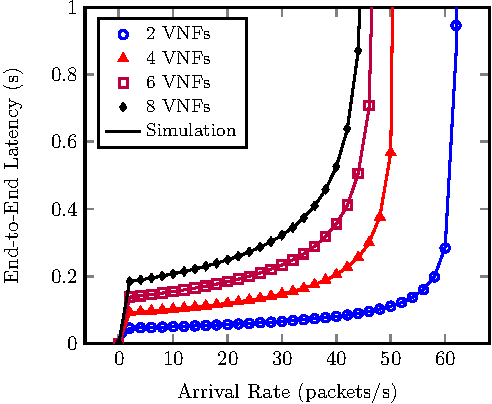
\includegraphics[width=\linewidth]{graphs/diff_lengths-crop}
		\caption{Latency predicted by the model and simulation for a single service with different lengths ($N_s=1$, $K_i={3,5,7,9}$, $k=4$, $k_v =2$, $p_m=0$).}
		\label{fig:length_chain}
	\end{minipage}
	\hfill
	\begin{minipage}[b]{.49\textwidth}
		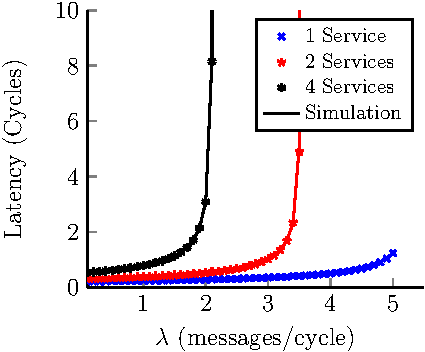
\includegraphics[width=\linewidth]{graphs/mult_services-crop}
		\caption{Latency predicted by the model and simulation for several services
		with different length service chains ($N_s={1,3,5}$, $K_i=3$, $k=4$, $k_v=2$, $p_m=0$).}
		\label{fig:mult_services}
	\end{minipage}

\end{figure*}

\section{Validation and Performance Analysis}
\label{sec:validation}

\subsection{Model Validation}

To verify the accuracy of the analytical model, a discrete event simulator has been built using OMNeT++ \cite{VargaH08} to simulate a NFV and SDN enabled datacentre network. Each simulation experiment was run until the network reaches its steady state where further network cycles do not change the collected statistics appreciably. In practice a datacentre can contain on the order of tens of thousands of servers \cite{AWS16}, with each switch supporting 1 to 100Gbits/s traffic a second. At high service rates, queue behaviour changes over very small intervals making it difficult to measure or demonstrate the accuracy of the results. Therefore, results from a scaled down version of a typical datacentre are presented in this work. Except where otherwise stated, the following parameters are used:

\begin{itemize}
	\item The number of ports $k = 8$, $k_{v} = 3$ and $p_{m} = 0$
	\item Each network component (switch/server, VNF and controller) can service 82 packets per second per port, \footnote{A 1Gb/s ethernet switch can process $\sim\!82000$ ethernet packets a second per port} ($\mu_{s}$, $\mu_{v}$ and $\mu_{c}$)
	\item Services are selected with equal probability
	\item The network provides 1 service with 5 VNFs ($N_s = 1$, $K_i = 5$)
\end{itemize}

Figs 2 to 5 depict the mean message latency predicted by the model plotted against those provided by the simulation experiments for a range of parameter settings. For the model, results are only shown where the network is in a steady state, i.e. where the arrival rate is lower than or equal to the service rate for all queues. The figures demonstrate that the simulation results closely match those predicted by the model. The tractability and accuracy of the analytical model make it suitable for analysis of next generation NFV and SDN enabled MCC datacentres.

\subsection{Performance Analysis}
We now show how the proposed analytical model can be a useful tool to optimise the design of an SDN and NFV enabled MCC datacenter network. We demonstrate the utility of the model for three key parameters: the scale of the network infrastructure, the table miss probability and the number and length of services.

\subsubsection{Impact of the size of the datacenter on the end-to-end latency}
The proposed analytical model can also be used to quantitatively analyse the relationship between latency and the size of the datacentre. From Fig. \ref{fig:num_ports} we can see that the Fat Tree scales as expected, with the increased number of VNFs in the network being balanced out by the increased service rate available at each switch. 

\subsubsection{Impact of the miss probability in SDN flow tables on the end-to-end latency}
The SDN paradigm provides the benefit of a simplified network management and centralised system optimisation. However, from the packet forwarding perspective, the centralised control incurrs extra transmission latency during packet delivery. The proposed analytical model allows us to investigate the relationship between the reliance on centralised control and the end-to-end latency of each service. Fig. \ref{fig:sdn_perc} shows that the system is only stable for low arrival rates when the SDN controller must frequently assist with routing instructions. Considering Eq. \ref{eq:arr_sdn}, we can see that the arrival rate at the SDN controller is proportional to the network traffic that is produced by the VNFs. Due to the total connectivity between the virtual machines and the SDN controller, even a slight increase of the traffic rate can overwhelm the SDN controller. To ensure that the SDN controller does not become a bottleneck in the system, network designers should ensure that routing tables at switches contain the majority of the information required for routing so that few requests must be sent to the controller, or ensure the processing capability of the SDN controller is sufficient to handle the traffic rate from the VNFs.

\subsubsection{Impact of the number and length of NFV services on the end-to-end latency}
Finally, we also consider the related situations of a different length services and of multiple services of varying lengths. As the datacenter network will be shared by multiple services to improve resource utilisation, it is important to investigate how these parameters impact the end-to-end latency. From Fig. \ref{fig:length_chain} we can observe the expected latency increasing as the length of the service increases. This is a consequence of the increased effective arrival rate that results from longer services (Eq. \ref{eq:effective_arrival}). In comparison, Fig. \ref{fig:mult_services} shows that increasing the number of services does not impact on the latency provided the expected arrival rate is distributed over the services. This indicates that the most important factor to consider when planning a datacentre is not the length or number of services, but the effective arrival rate of these two properties combined.

% !TeX root=main.tex

\section{Conclusion}
\label{sec:conclusions}
% Outline paper again
Emerging services will place intense demand on the datacentre. To provide a good service whilst remaining economically viable, modern datacentres are exploring the potential of SDN and NFV to provide efficient allocation of resources and simplify management. Whilst these are often considered complementary technologies, previous analytical models in the literature have typically considered them in isolation. Further previous work on this topic has not considered the importance of the interconnection network or how multiple services with different length service chains may affect performance.

In this paper we have presented a comprehensive analytical model capable of modelling an SDN and NFV enabled datacentre. Extensions are derived that accurately model how the presence of multiple services with varying length service chains impacts the datacentre. Finally useful properties pertaining to the performance of the network are derived from the mathematical model. These show that the edge switches, virtual switches and SDN controller can receive disproportionately more traffic than the other components in the datacentre.

\bibliographystyle{IEEEtran}
\bibliography{IEEEabrv,bibliography}

\end{document}